\documentclass{article}

\usepackage{hyperref}
\usepackage{graphicx}

\title{Final Report}

\author{
James Atwood and Luis Pineda \\ % alphabetical order
}

\begin{document}
\maketitle

\section{Introduction}
Our project was a
submission\footnote{\url{https://github.com/luisenp/sigmod14}} to the
SIGMOD 2014 programming challenge.  In this competition teams are
provided with a large (relational) social network dataset and are
asked to implement four queries related to the graph structure of the
data. The motivation for choosing this project was
twofold; first, there is a large (and quickly increasing) volume of
graph-structured data available today, and second, developing
efficient mechanisms for representing and querying graph data is a
challenging research problem that is currently the subject of
considerable interest in the database community.

Using a relatively simple design and incremental optimization,
we were able to complete our Java implementation by the April 15th
deadline and submit it for evaluation.  According to the
leaderboards\footnote{\url{http://www.cs.albany.edu/~sigmod14contest/leaders.html}
  under team name `shparg'}, which provide preliminary results, our
entry ranks 22nd out of 32 total submissions (see Figure
\ref{fig:leader}).  Unfortunately, the final evaluation on held-out
data will not be released until after this report has been written, so
we can not report our official standing.



\begin{figure}[t]
  \centering
  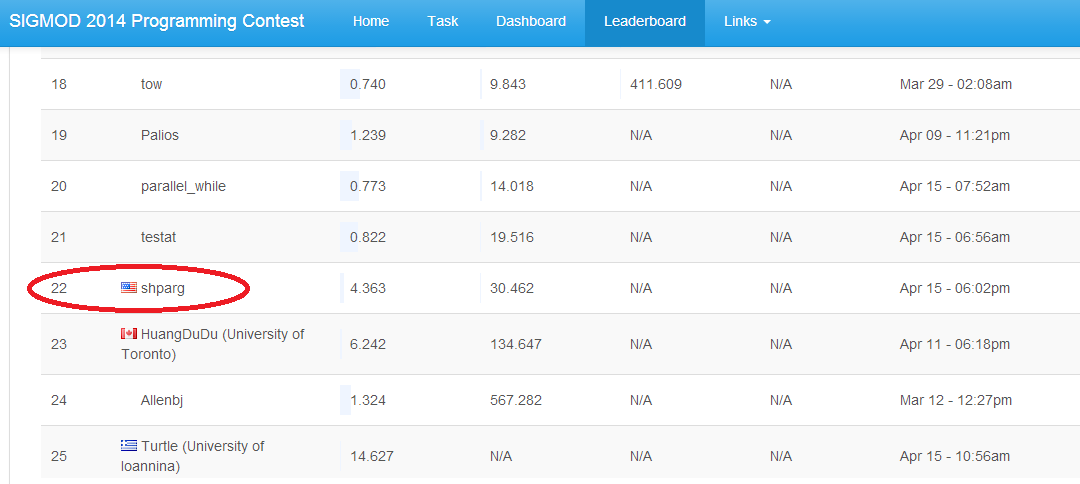
\includegraphics[scale=0.45]{img/leaderboard.png}
  \label{fig:leader}
  \caption{Final position of our team `shparg' in the SIGMOD programming challenge.}
\end{figure}

\section{Background and Related Work}
\subsection{Challenge Description}

\subsubsection{Data}
We are provided with a relational dataset which describes a social
network.  Example entities include people, interest tags and places, 
and example relations include `person knows person', `person works at place'
and `person has interest in tag'.  Each entity and
relationship is stored as a pipe-delimited file.  Entity files are
named after the entity type (e.g. `person.csv') and contain features.
Relation files are named after the relation they contain
(e.g. `person\_knows\_person.csv') and contain pairs of entities which
have that relation.

\subsubsection{Task}
The task is to return the correct results of a provided set of queries
against the provided data as quickly as possible.  Performance is
first measured by correctness (if any query results are incorrect, a
submission is invalid) followed by runtime (with lower being better).
`Runtime' means the wall-clock time from program initiation to
termination.  Note that subtasks like reading the data into memory or
constructing an index will factor in to the runtime.

\subsection{Query types}
There are four types of queries that need to be answered.

\subsubsection{query1(p1, p2, x)}
Given two integer person ids p1 and p2, and another integer x, find
the minimum number of hops between p1 and p2 in the graph induced by
persons who
\begin{enumerate}
\item have made more than x comments in reply to each others'
comments, and
\item know each other.
\end{enumerate}

\subsubsection{query2(k, d)}
Given an integer k and a birthday d, find the k interest tags with the largest range, where the range of an interest tag is defined as the size of the largest connected component in the graph induced by persons who
\begin{enumerate}
\item have that interest,
\item were born on d or later, and
\item know each other.
\end{enumerate}

\subsubsection{query3(k, h, p)}
Given an integer k, an integer maximum hop count h, and a string place
name p, find the top-k similar pairs of persons based on the number of
common interest tags. For each of the k pairs mentioned above, the two
persons must be located in p or study or work at organizations in
p. Furthermore, these two persons must be no more than h hops away
from each other in the graph of people who know each other.

\subsubsection{query4(k, t)}
Given an integer k and a string tag name t, find the k persons who
have the highest closeness centrality values in the graph induced by
persons who
\begin{enumerate}
\item are members of forums that have tag name t, and
\item know each other.
\end{enumerate}


\subsection{Related Work}
Traditionally, research in databases has focused on the relational
model first proposed by Codd \cite{codd1970relational}.  This model
becomes awkward and inefficient when applied to graph data
\cite{rodriguez2011graph}, particularly for queries related to
complex structure (i.e., requiring more than nearest neighbors).  For
an example, please see \cite{he2008graphs} (Figures 1 and 2).  More
recent work has proposed other data models and query languages that
more appropriately capture the rich structure evident in graph data;
for instance,
\cite{he2008graphs,sun2012efficient,low2010graphlab} (see
\cite{angles2008survey} for a survey of recent graph database
models).  

%However, much of this work is task oriented; for example, a system
%may optimize for path-related queries at the expense of subgraph
%isomorphism.  For the task at hand, it is unclear which existing
%technologies, if any, provide the best performance for the queries of
%this challenge.

\section{Implementation}
\subsection{Overall Approach}
We divided the challenge into two subtasks: first, read and index all
of the data that is required to answer the queries (the `reading
phase'); then, perform the queries and output results (the `query
phase').  We found that both tasks' runtime was on the same order of
magnitude.  

\subsection{Data Representation}
\subsubsection{Embedded Database Design}
Originally, we designed our implementation around the open-source
Neo4j\footnote{\url{http://www.neo4j.org/}} disk-based graph database
system.  We thought this system was appropriate because the queries in
the challenge are largely path-oriented, and it seemed unlikely that
all of the relevant data would fit in memory\footnote{Although we
  later found that we could, in fact, fit the relevant data in
  memory.}.  Neo4j makes use of the \emph{ADI} index structure
\cite[Chapter~6]{IanRobinson:2013ul} described in
\cite{wang2004scalable}, which is designed to facilitate efficient
edge support checking (that is, quickly finding edges) and adjacent
edge checking (that is, quickly finding edges that share a node).
This index structure seemed well-suited to the task at hand because it
allows a graph on disk to be efficiently queried with regards to path.

Our implementation of this approach performed very poorly, however.
An implicit assumption of this design was that the high initial cost of
populating the graph database would be amortized over the large number
of queries against the data.  Instead, we found that the runtime cost 
of reading and indexing the data using Neo4j was prohibitively large,
and any potential improvement Neo4j could offer in query performance
would not offset the cost of populating the database.
It seemed likely that this undesirable behavior will be found
with other database systems; if fixed setup costs are amortized over
the lifetime of a database system measured in years, the cost of
establishing the database is trivial, so reducing this cost is likely
not a design goal.  So, we abandoned the embedded database approach.

\subsubsection{In-Memory Design}
We turned our attention to a simpler key-value approach tailored to
the SIGMOD challenge dataset.  Specifically, we indexed nodes and
edges via several simple in-memory arrays and hash tables, with one
structure for each type of node or edge relevant to the queries.  This
design choice was motivated by an analysis of the provided datasets
(1k and 10k persons), which suggested that most of the storage needs
are due to nodes that need not persist through the query phase;
examples include comments and forums. This information is required to
persist only while the database is populated; for instance, comments
nodes are required to compute the number of comments between people,
but are not needed thereafter.  

We confirmed on the SIGMOD system that
this design could hold a 100k person dataset in memory without
exceeding the 15Gb of available memory. Moreover, the in-memory approach 
reduced the time it took to both index the data and answer the queries 
by several orders of magnitude with respect to our initial Neo4j implementation.  Thus, 
we accordingly moved forward with the in-memory design.

%Moreover, during the
%actual contest it became clear that the running time of the more
%difficult queries (in particular query4) was the real bottleneck, so
%the final simple design was largely motivated by attempting to solve
%all queries on the 100k dataset after the data was completely loaded
%in memory.

%Accordingly, we propose the following approach.  Our primary data
%abstraction will be an adjacency matrix over the nodes which
%constitute a network.  The nodes will themselves be an interface for
%the data provided by the challenge.  We will be investigating the
%particulars of the implementation of the adjacency matrix and node
%abstractions throughout the project. To be more concrete, a node could
%be an object representing a person, with fields for attributes like
%gender and age.  Or, a node could simply be a pointer to a query which
%retrieves the node's data from disk.  The adjacency matrix could be a
%simple $n$ by $n$ array, where $n$ is the total number of people in
%the dataset.  This adjacency matrix representation scales poorly; we
%will probably need to employ some sparse representation or other
%compression mechanism to maintain this structure in memory, or
%implement some mechanism for managing adjacency matrices that are only
%partially stored in memory, such as the \emph{ADI} structure described
%in \cite{wang2004scalable}. Finally, after developing appropriate
%implementations of the node and matrix abstractions, we will focus on
%developing efficient indexing and graph traversing mechanisms for
%servicing the four types of query that are the subject of the SIGMOD
%challenge.

%Neo4j is a Java system, so our implementation language will be Java.
%We will use the embedded interface of
%Neo4j\footnote{\url{http://docs.neo4j.org/chunked/stable/tutorials-java-embedded.html}}
%in order to construct an indexed graph database from the provided
%data.  This database will be constructed and queried using the Core
%API, which provides the lowest user-level abstractions in the Neo4j
%system, and is generally faster than the higher-level Traversal and
%Cypher APIs \cite[Chapter~6]{IanRobinson:2013ul}.

%The following pseudocode demonstrates how we will use the disk-based
%system to perform the first query, which finds the shortest path
%between two people p1 and p2 who have replied to each other's comments
%at least x times.


%More specifically, our implementation language will be Java.  The
%adjacency matrix representation will initially be implemented as a
%sparse Colt
%matrix \footnote{\url{http://acs.lbl.gov/software/colt/api/cern/colt/matrix/package-summary.html}}.


\subsubsection{Data structures and indexes}
Our Java implementation of the in-memory design defines the following
data structures for each of the relevant entities in the contest data.

\begin{itemize}
\item \textbf{Person} stores a 32-bit integer representing the person's id, a 64-bit integer representing the person's birthday, a list of tag interests, a list of locations the person lives, works or studies at, and a hash map of known persons and the replies given to each of them.
\item \textbf{Tag} stores a 32-bit integer representing the tag's id, a string representing the tag name, a hash set of persons interested in this tag and a hash set of persons interested in this tag through a forum membership. 
\item \textbf{Forum} stores a 32-bit integer representing the forum's id and a list of tags this forum is associated with.
\end{itemize}

For each entity in the social network we create an instance of the corresponding data structure. Each type of entity is stored in its own in-memory table, which is indexed by the 32-bit id. In the case of the persons table, since the datasets always include all persons ids in the rage (e.g., ids 0 to 9,999 for the 10k dataset) we used a pre-allocated array of size 100k with a one to one mapping between the id and the array index; this lead to faster data loading and query response times. For all other entity types, we used hash maps indexes. 

Additionally, we stored the following relationship tables: 

\begin{itemize}
\item \textbf{commentCreator} stores the 32-bit id of the person who created each comment, indexed by a 32-bit comment id. It is essentially an array where index \emph{i} stores the id of the person that created the comment with id \emph{i}. It's pre-allocated to a size of 700,000,000 comments, which is enough for the 100k dataset used in the SIGMOD preliminary evaluation. 
\item \textbf{placeOrg} is a hash map that stores the place a given organization is located at.  
\item \textbf{placeLocatedAtPlace} is a hash map that stores the place a given place is located at (e.g., Amherst is located in Massachusetts).  
\item \textbf{namePlaces} is a hash map that stores the ids of all places with a given name. Note that different places (i.e., with different ids) can have the same name string.
\end{itemize}

These tables are populated by reading files such as person.csv,
comments.csv, tags.csv, comment\_hasCreator\_person.csv and so forth.
Most of the memory consumption is due to the \texttt{commentCreator}
table.  However, this table is only used temporarily during data
loading, to obtain the number of replies between people. The table
\texttt{commentCreator} is cleared after these numbers are stored in
the persons table so that freed memory can be used for other parts of
the dataset.

\subsection{Query Implementations}

We implement each query as a graph algorithm over the graph defined by
the indexed data.

\subsubsection{Query1}
We solve Query 1 via a bidirectional breadth first search (BFS) of the
person-knows-person graph based on the constraint on number of replies
x.  The hash map of neighbors stored by each person instance can be used
to quickly prune edges that don't satisfy the constraint. 

\subsubsection{Query2}
We add all tags to a priority queue where the order of
the tags is based on the size of the largest connected component of
the induced graph. To compute the connected components, we use the list of persons 
that are interested in the tag, and information about the birthday stored 
by each person node. We use this information to create the induced graph on-the-fly 
and then compute the size of the largest connected component using several BFS.
              
\subsubsection{Query3} 
First, \texttt{namePlaces} is used to find all places with
the given name. For each of these places p, we perform a linear scan to find 
all persons located at p and add these persons to the induced graph. 
To check if a person is located at p, we use both the 
list of places stored by the person node, but also the table 
\texttt{placeLocatedAtPlace} to recursively check if any place 
in the induced hierarchy is contained in p. If at least one does, 
the person is added to the induced graph.
              
When all the relevant persons are added to the graph, 
the similarity score of all possible pairs of persons in this
graph is computed and these are added to a priority queue. To speed up
the similarity computation we use the hash set of persons interested in
each tag (where the hash is given by person id). Therefore the similarity 
between two persons can be computed in linear time in the number of 
interest tags.
              
\subsubsection{Query4} First a linear search is used to find the tag with
the given name. Then the induced graph of persons that are member of
forums with this tag is created, using the list stored by each \texttt{Tag} instance.
               
On the induced graph the centrality score of each person p is computed
using a BFS. Every time a node is expanded during a BFS for person p, the
algorithm checks if the best possible centrality p can
achieve (given the nodes expanded so far and their distances) 
is smaller than the k-th best centrality seen so far (using a priority queue). 
If it is, the BFS is stopped and person p can be ignored. 

In our final submission we used an approximate version of this algorithm
in which person nodes are first sorted by non-increasing node degree in the 
induced graph. Then we only considered the top $25\%$ of the nodes as 
candidates for top k centrality nodes. This worked well on both the 1k and 10k
datasets and reduced computation time significantly (see Figure \ref{fig:results}).
However, there are no guarantees of correctness. 

In a subsequent version (developed after the SIGMOD deadline), 
we sorted persons by the number of persons they can reach within at most 
two steps, and considered only the top $5\%$. This worked very well on the 
10k dataset, significantly reducing the time it takes to solve Query 4. 
However, it did not work on the 1k dataset. Nevertheless, it 
should be possible to devise an exact version of this strategy based on some
incremental pruning of approximate centrality computations. 

\subsection{Concurrency}
To take advantage of the eight cores provided by the SIGMOD system, we developed a 
multi-threaded implementation of the query solver. Since the challenge involves 
answering hundreds of queries, the easiest (and possibly best) way to take 
advantage of parallelism is to cleverly distribute queries between different
threads, instead of developing complex multi-threaded implementations of each 
query. 

In our final design, queries are uniformly distributed between eight
threads, under the assumption that all queries take approximately the
same time to compute. This is true for our last approximate
implementation of query 4, although not for previous
implementations. In previous versions, type 4 queries were orders of
magnitude more costly than the other query types. Thus, we also
developed some versions in which two threads are exclusively dedicated
to answer type 4 queries and the remaining threads to other query
types.  It is worth mentioning that we also experimented with a
multi-threaded version of q	uery 4, although we didn't obtain any
significant computational savings from this version.

%\subsection{Concurrency}
%We introduced concurrent behavior in order to take full advantage of
%the multi-core test system (which is described in section
%\ref{sec:results}).  All concurrent behavior took place in the query
%phase.  Specifically, the queries were distributed evenly among
%available cores and run concurrently, and within queries of type four,
%the centrality of each individual was computed concurrently.

\section{Results}
\label{sec:results}
\begin{figure}
  \centering
  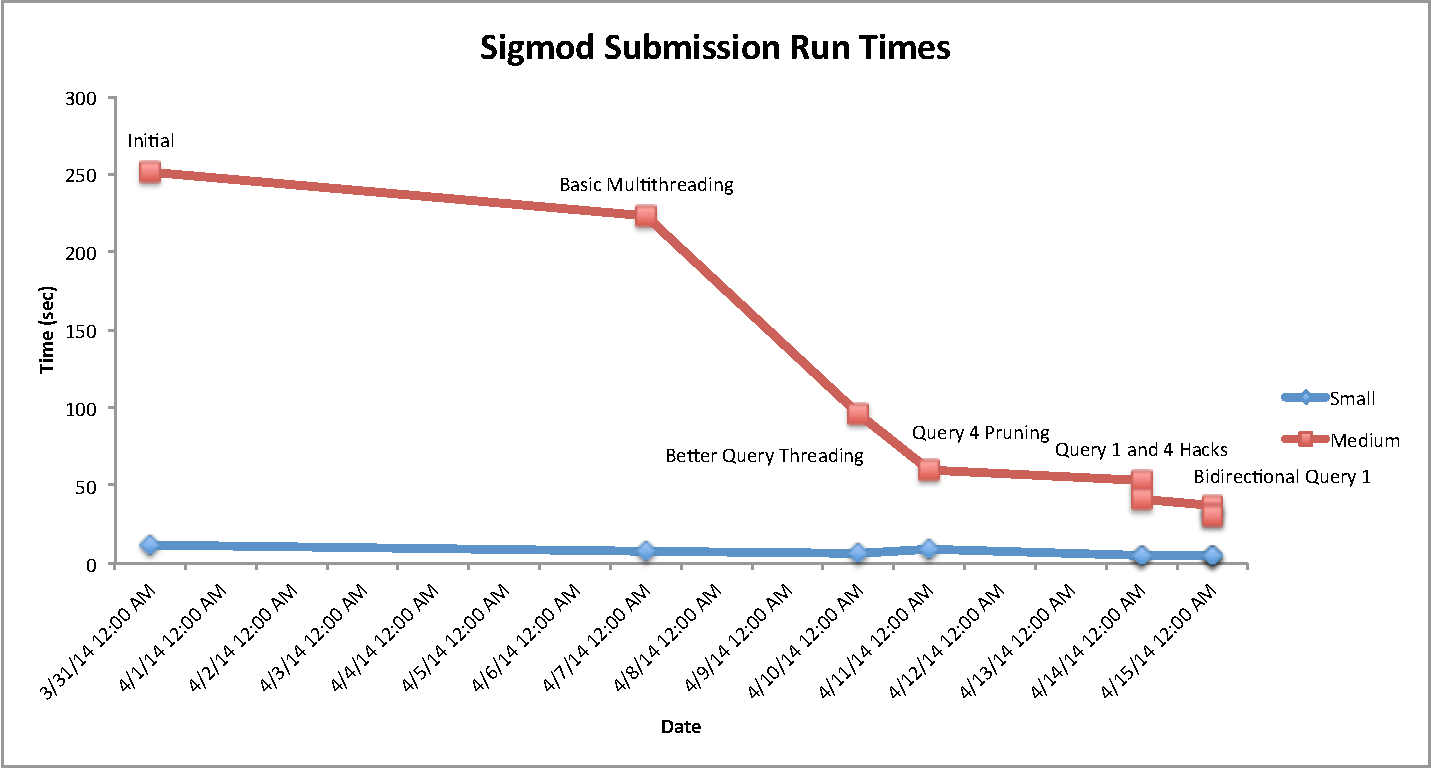
\includegraphics[scale=0.5]{img/results.pdf}
  \label{fig:results}
  \caption{Evolution of the performance of our implementation on the
    SIGMOD system.  The horizontal axis gives the date of the
    submission and the vertical axis shows the runtime as
    reported by the submission system.  Each submission is annotated
    with the optimizations that were introduced with it.  `Medium'
    indicates the dataset with 10,000 people and `Small' the dataset
    with 1,000 people.}
\end{figure}

Our implementation's performance is shown in Figure \ref{fig:results}.  All times were provided by the SIGMOD submission system (measured in seconds).  According to the challenge description\footnote{\url{http://www.cs.albany.edu/~sigmod14contest/task.html}}, performance was measured on a server with the following specification:
\begin{itemize}
\item Processors: Two 2.67 GHz Intel Xeon E5430 (4 cores each, 8 cores total)
\item Main Memory: 15 GB
\item OS: Red Hat Enterprise Linux Server 6.5 (Santiago) 
\item Java: JDK 1.7.0
\end{itemize}

\section{Discussion}
Our implementation was about an order of magnitude slower than the
best submission to SIGMOD.  We speculate that we could have increased
performance as follows:

\subsection{Improved Concurrency}
We did not introduce any concurrency into the process of loading the
data.  This could have improved performance significantly given that
large portion of running time that loading took.  Furthermore, the
computation of some queries could have been initiated before all data
was loaded.

\subsection{Further Investigation of Heuristics}
We found that the introduction of a simple heuristic to the query 4
implementation significantly improved the runtime of the entire
pipeline; namely, sorting person by non-increasing node degree in the
then we only considered the top $25\%$.  After the contest, we found
that sorting persons by two-step reachability and reducing the
considered persons to the top $5\%$ yielded additional savings.  While
these heuristics did not guarantee correctness, they were correct in
practice.  The introduction of other simple heuristics or more complex 
algorithms for computing graph measures in large networks 
could have provided more benefit (e.g., \cite{okamoto2008ranking,potamias2009fast}).

\subsection{Implementation Language}
We found that performance increased when we avoided `boxed' Java
types; that is, fundamental types (like int) performed better than
objects (like Integer).  This suggests that a lower-level language,
such as C, could have yielded performance benefits.

\section{Conclusion}
We developed a simple in-memory approach for performing the
graph-related queries of the SIGMOD challenge.  We found that more
complex representations, such as an embedded graph database, performed
quite poorly when the time to load and index the data is taken into
consideration.  Given the challenge constraints, a simple in-memory
approach based on arrays and hash indices offered reasonable
performance for the full challenge pipeline, and our submission was
(preliminarily) ranked 22nd out of 32 total submissions.


%Overall, we are currently ahead of the schedule we proposed; all queries are implemented and we have submitted an implementation to SIGMOD.  Our results can be seen on the
%leaderboard\footnote{\url{http://www.cs.albany.edu/~sigmod14contest/leaders.html}} under team name `shparg'.
%
%Progress on Project Milestones:
%\begin{itemize}
%\item Early March: Download datasets; setup Neo4j library;
%  design of pipeline; implementation of queries 1 and 2 on small test dataset. \textbf{DONE}
%\item March 20th: Implementation of queries 3 and 4 on small test dataset. \textbf{DONE}
%\item April 1st: Submit midterm report. \textbf{DONE}
%\item April 8th:  Run experiments with the larger dataset. \textbf{DONE} \\Refine the implementation to address scalability issues.
%\item April 15th: Submit system to SIGMOD if we have a competitive entry. \textbf{DONE}
%\item April 29th: Present results to class.
%\item May 8th: Final report.
%\end{itemize}
%
%We will devote our remaining time to improving performance and
%addressing scalability issues.  Our main idea is to use a disk-based
%extensible hash to index the nodes and edges over the original
%(unsorted) heap files\footnote{which implies we will be using
%  Alternative 3 for the index data entries.} so that we may avoid
%loading the entire dataset into memory.  This index is appropriate
%because we are only concerned with equality searches. 
%
%Additionally, we are going to add multi-threading capabilities to our
%system, in order to take advantage of the 8 cores available on the SIGMOD computers. 
%Since all queries can be answered independently are no data is added after 
%the initial database population, implementing multiple threads should 
%be straightforward.

\newpage

\bibliographystyle{abbrv}
\bibliography{final}

\end{document}
